\documentclass{ncc}
\usepackage[utf8]{inputenc}
\usepackage[russian]{babel}
\usepackage[T2A]{fontenc}
\usepackage{amssymb}
\usepackage{amsmath}
\usepackage{pscyr}
\usepackage{graphicx}
\usepackage{listings}
\usepackage{hyperref}

\lstloadlanguages{C}
\lstset{
language=C,
extendedchars=\true, %Чтобы русские буквы в комментариях были
% inputencoding=utf8,
commentstyle=\it,
stringstyle=\bf,
belowcaptionskip=5pt }
\title{Дифракция и шейдеры}

\begin{document}
\maketitle
\tableofcontents

\section{Дифракция}

\textit{Дифракция} -- это явление, связанное с волновой природой света. Свет, будучи
волной, может огибать препятствия и оказываться в области геометрической тени.
Например, если взять источник света и непрозрачный экран с квадратным
отверстием, то на стене за экраном мы увидим вместо квадрата вот такую картину:
\begin{figure}[h!]
\center
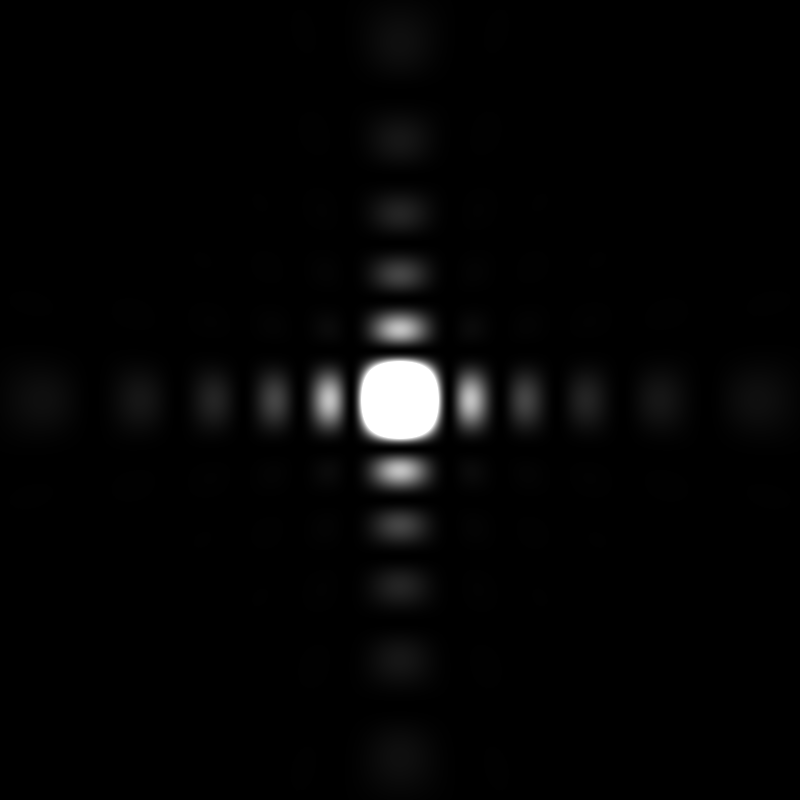
\includegraphics[width=.35\textwidth]{2015-10-12-difraction-square.png}
\caption{Дифракция на квадратном отверстии}
\end{figure}

Для понимания этого явления сначала стоит познакомиться с \textit{интерференцией}.

\section{Интерференция. Опыт Юнга}
\textit{Интерференцией} называют взаимное усиление и ослабление волн при их наложении. Опыт Юнга отлично демонстрирует это
явление.
Сделаем в непрозрачном экране две щели, с одной стороны поместим источник света, а с другой -- экран, на котором будем наблюдать интерференцию:
\begin{figure}[h]
\center
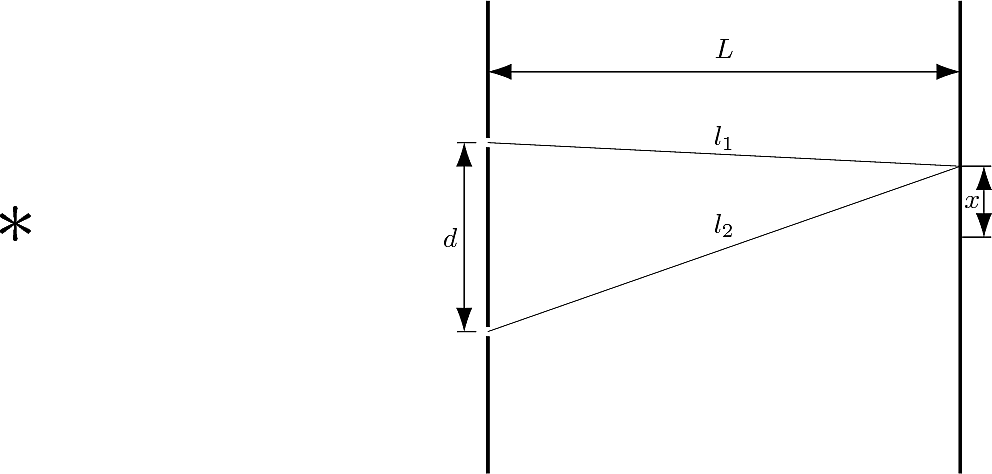
\includegraphics[width=\textwidth]{2015-10-12-difraction-exp.png}
\caption{Схема опыта Юнга}
\end{figure}

При этом вблизи центра экрана мы будем наблюдать полосы:
\begin{figure}[h!]
\center
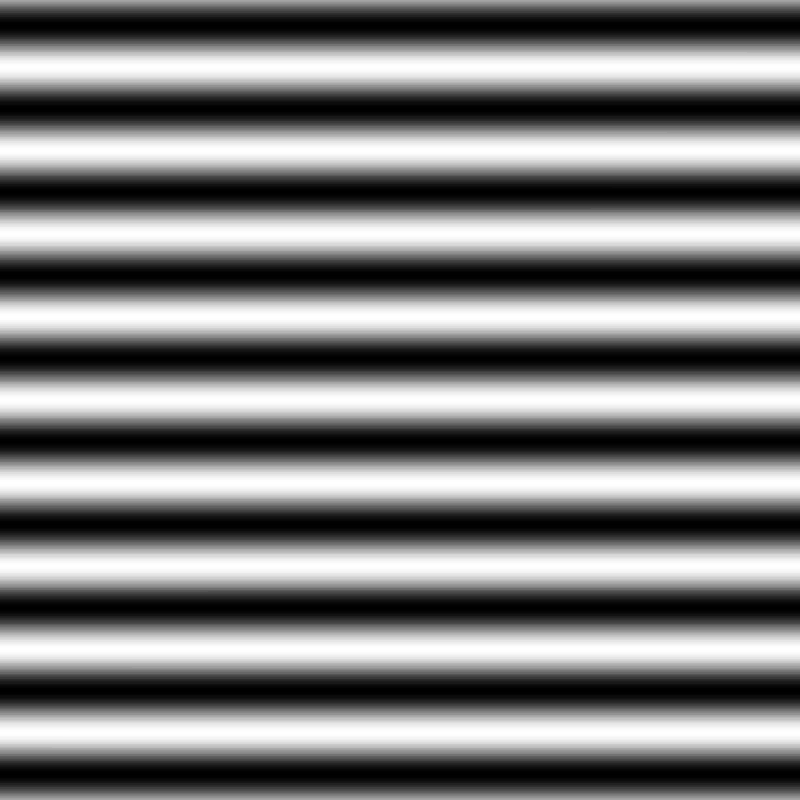
\includegraphics[width=.2\textwidth]{2015-10-12-difraction-young.png}
\caption{Интерференционнаяя картина в опыте Юнга}
\end{figure}

Теоретически это можно обосновать следующим способом. Свет -- электромагнитная волна, поэтому на экране поля от двух щелей будут складываться
\[
    A = a_1 e^{i(kl_1 - \omega t + \phi_1)} + a_2 e^{i(kl_2 - \omega t + \phi_2)}.
\]
Для простоты положим амплитуды волн равными, а их начальные фазы нулевыми. Тогда
\[
    A = 2a e^{i\left(\frac{k(l_1+l_2)}{2}-\omega t\right)} \cos\frac{k(l_1-l_2)}{2}.
\]
Зная распределение амплитуды перейдём к интенсивности:
\[
    I = 4I_0\cos^2\frac{k(l_1-l_2)}{2}, 
\]
где \( I_0 \) -- интенсивность света на экране от одной из щелей.
\begin{figure}[h!]
    \center
    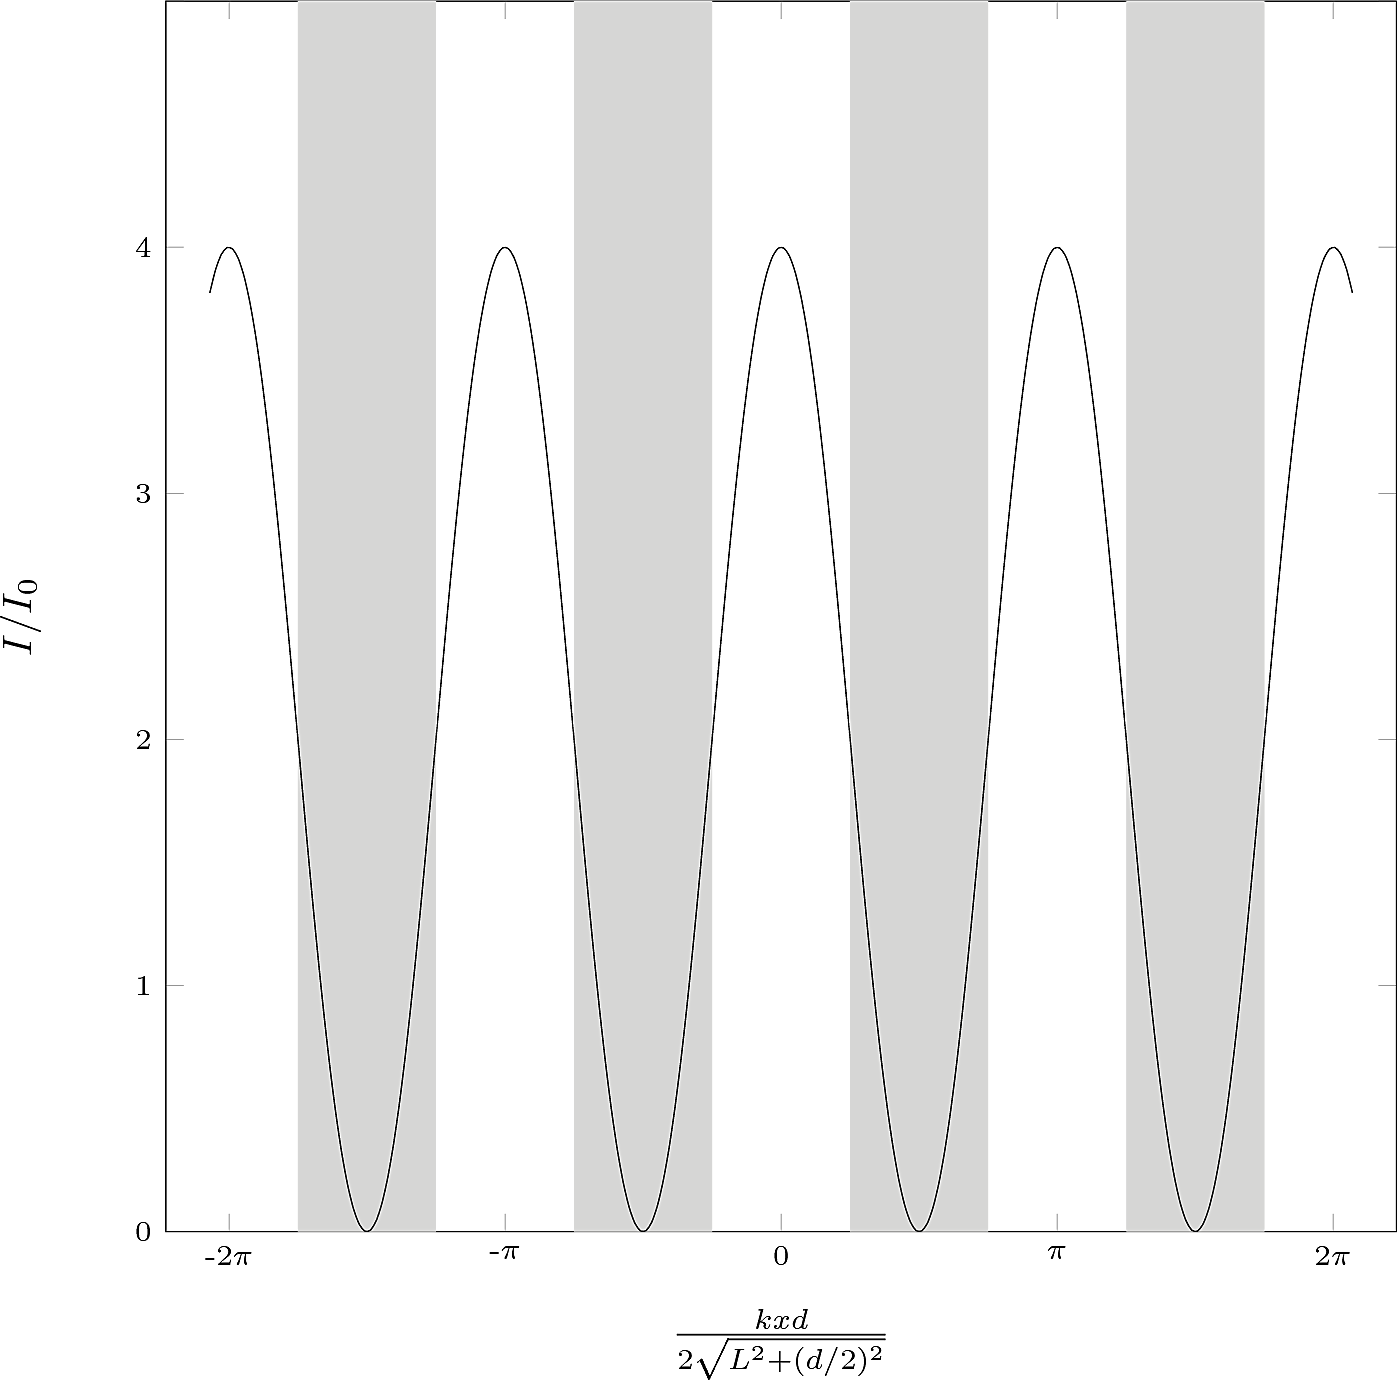
\includegraphics[width=.7\textwidth]{2015-10-12-difraction-inter.png}
    \caption{Распределение интенсивности вблизи центра экрана в опыте Юнга}
\end{figure}
\[
    l_1 = \sqrt{L^2 + (d/2 - x)^2},\quad l_2 = \sqrt{L^2 + (d/2 + x)^2},
\]
\[
    l_1 - l_2 = \sqrt{L^2 + (d/2 - x)^2} - \sqrt{L^2 + (d/2 + x)^2} = -\frac{2xd}{l_1 + l_2}.
\]
Вблизи центра экрана \( x \ll L \), поэтому
\[
    l_1 + l_2 \approx 2\sqrt{L^2 + (d/2)^2},
\]
\[
    I = 4I_0\cos^2\frac{kxd}{2\sqrt{L^2 + (d/2)^2}}. 
\]


Дифракция -- это интерференция от большого числа источников.

\section{Построение интерференционной картины}
Задача построения интерференционной картины очень хорошо параллелится -- ведь
освещённость различных точек экрана рассчитывается независимо.

Напишем простенький шейдер, иллюстрирующий интерференционную картину в опыте Юнга:

\begin{lstlisting}
// young.glsl

#version 130       // версия glsl

out vec3 color;

void main() {
    float d = 4e2;
    float l = 5e5;
    // получаем координату точки на текстуре
    float x = 6e4 * (gl_TexCoord[0].y - 0.5);
    float lambda = 5.0;
    float k = 2.0 * 3.15159 / lambda;
    float phi1 = k * length(vec2(l, x - d / 2.0));
    float phi2 = k * length(vec2(l, x + d / 2.0));
    vec2 amplitude = vec2(cos(phi1) + cos(phi2),
                          sin(phi1) + sin(phi2));

    amplitude /= 2.0;
    float intensity = dot(amplitude, amplitude);
    color = vec3(intensity);
}
\end{lstlisting}

\section{Построение дифракционной картины}
Теперь можно перейти к построению дифракционной картины. Вернёмся к дифракции на квадратном отверстии. Каждую точку квадрата можно рассматривать как точечный источник. Так как в квадрате бесконечно много точек, то разобьём квадрат сеткой на малые части и, считая каждую точечным источником, посчитаем их суммарную амплитуду и интенсивность. Считая, что квадрат равномерно освещён параллельным пучком, а ячейки сетки имеют равные площади, получаем
\[
    A \sim \sum\limits_i \frac{e^{ikl_i}}{l_i},\quad I = \langle A^2 \rangle = \frac{|A|^2}{2}.
\]
Эти величины уже можно посчитать численно при помощи шейдера:
\begin{lstlisting}
// square.glsl

#version 130       // версия glsl

out vec3 color;

void main() {
    int n = 40;
    float a = 4e1;
    // получаем координату точки на текстуре
    vec3 p = vec3( 10e4 * (gl_TexCoord[0].xy - 0.5), 5e4);

    float lambda = 5.0;
    float k = 2.0 * 3.15159 / lambda;
    vec2 amplitude = vec2(0.0);
    for (int i = 0; i < n; ++i)
        for (int j = 0; j < n; ++j) {
            vec3 source = vec3(a * (float(i) / float(n-1) - 0.5),
                               a * (float(j) / float(n-1) - 0.5), 0);
            float phi = k * length(p - source);
            amplitude += vec2(cos(phi), sin(phi));
        }

    amplitude /= float(n*n/4.0);
    float intensity = dot(amplitude, amplitude);
    color = vec3(intensity);
}

\end{lstlisting}
На выходе получается уже знакомая картина:
\begin{figure}[h]
\center
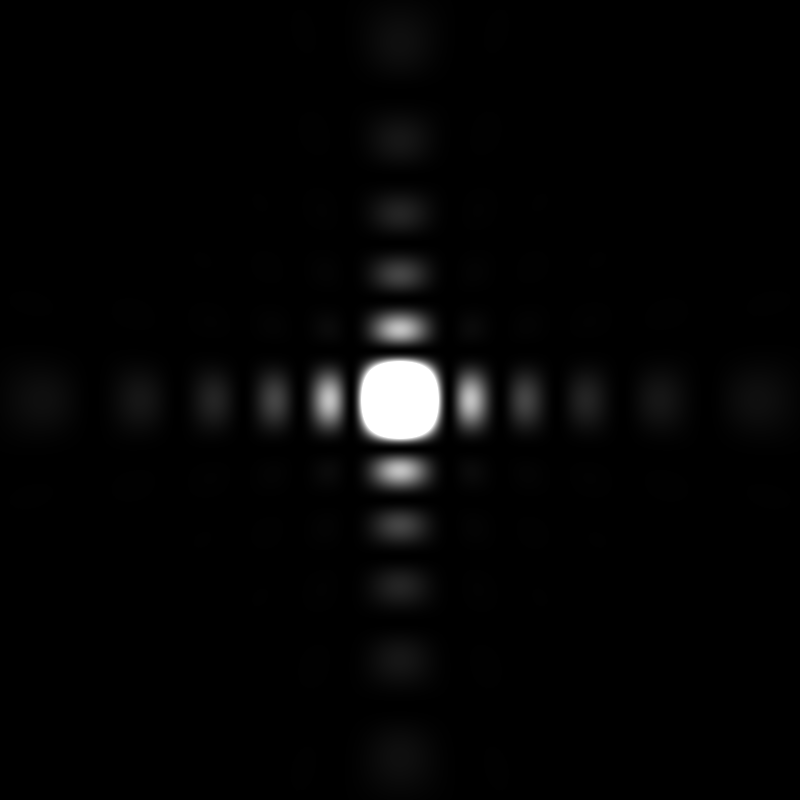
\includegraphics[width=.3\textwidth]{2015-10-12-difraction-square.png}
\caption{Дифракция на квадратном отверстии}
\end{figure}

При помощи той же техники можно получить дифракционные картины на отверстиях более интересной формы:

\begin{figure}[h!]
\center

\includegraphics[width=.3\textwidth]{2015-10-12-difraction-circle.png}
\hfil
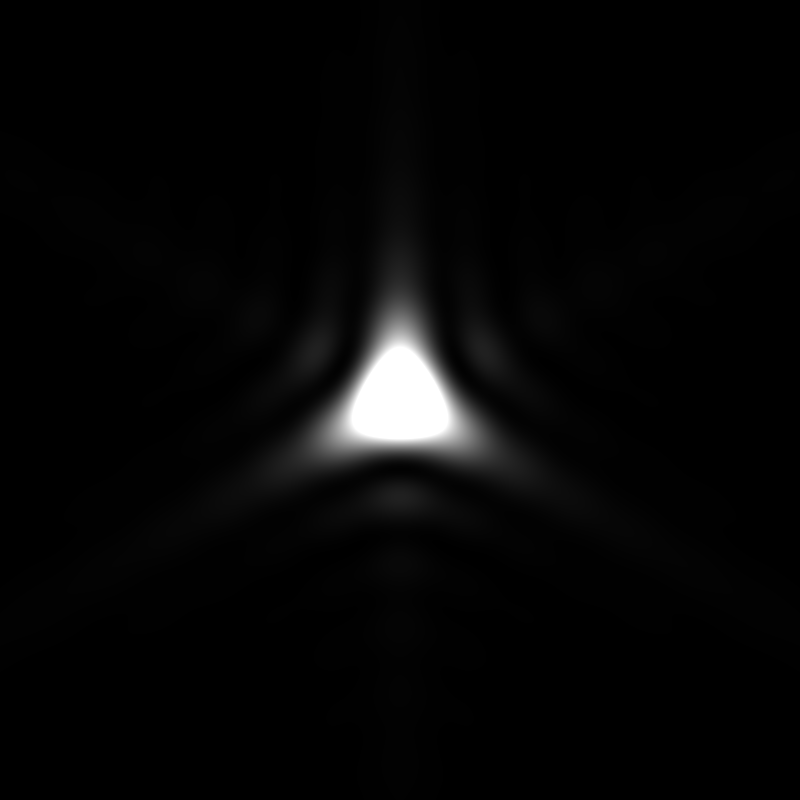
\includegraphics[width=.3\textwidth]{2015-10-12-difraction-triangle.png}
\caption{Дифракция на круглом и треугольном отверстиях}
\end{figure}

Код \href{https://github.com/citrux/difraction}{здесь}.
\end{document}
